
\section{Versions released in 2007 (26)}
\subsection{1.19.4.7 (Dec/23/2007)}

\begin{itemize}
  \item \textit{Application option} was a bit improved.
    Now, it is posssible to
    set Tinn-R to close previous instance of the viewer (PDF or DVI) in
    the \textit{Processing/Latex/More} options.
    Makes it easier to compile under Latex, as Miktex will
    not gives the message: \texttt{I can't write the file ...} in the
    DOS prompt. Note that \texttt{any instance of the viewer (if opend)}
    with the caption \texttt{'FileBeeingCompiled'.pdf} will be closed.
\end{itemize}


\subsection{1.19.4.6 (Dec/17/2007)}

\begin{itemize}
  \item A very simple splash screen was added to application starting.
  \item The functionality of \textit{Latex/Accents} was improved.
    Now if you have a selection in the editor it will be filled
    inside the brackets '\{\}', otherwise, the simple accent
    will be inserted.
\end{itemize}


\subsection{1.19.4.5 (Dec/14/2007)}

\begin{itemize}
  \item Bug(s) fixed:
    \begin{itemize}
      \item A couple of bugs related to the prior version
        \textit{1.19.4.4 (Dec/13/2007)} were fixed.
    \end{itemize}
  \item Parts of the source code were optimized.
\end{itemize}


\subsection{1.19.4.4 (Dec/13/2007)}

\begin{itemize}
  \item The appearance of the \textit{Latex symbols} now have a better layout,
    alphabeticalilly ordered. The structure of ini file, related with to it,
    was also changed.
  \item This version enables the user to set two comment(s) character(s): the
    main (used for all syntax) and to latex. The options were added to the main
    menu \textit{Format/Block}: it is possible to \textit{comment all},
    \textit{uncomment first} and \textit{uncomment all}. The
    \textit{Application options} was a bit reworked to allow the user to
    set the preferred latex comment (\%, \%\%, \%\%\%, etc).
  \item Some default shortcuts were changed. The \textit{ini file related}
    will be updated to reflect these changes and a backup of the old
    resource file will be made at first use of this version.
\end{itemize}


\subsection{1.19.4.3 (Dec/12/2007)}

\begin{itemize}
  \item Bug(s) fixed:
    \begin{itemize}
      \item A bug related with the new resource \textit{Count} in
        latest version \textit{1.19.4.2 (Dec/11/2007)} was fixed.
    \end{itemize}
  \item The tool \textit{Markup/Latex} was improved.
  \item \textit{Latex Itemization and Enumeration} procedures were
    a bit improved.
  \item The color of the \texttt{matched brackets} are now user
    configurable. Set it at
    \textit{Options/ Syntax and colors/ Preferences/ Brackets(FG)}.
\end{itemize}


\subsection{1.19.4.2 (Dec/11/2007)}

\begin{itemize}
  \item The tool \textit{Markup/Latex} was improved by adding a toolbar.
  \item Parts of the source code were optimized.
  \item The \textit{Application options} interface was a bit reworked.
\end{itemize}


\subsection{1.19.4.1 (Dec/01/2007)}

\begin{itemize}
  \item Bug(s) fixed:
    \begin{itemize}
      \item A couple of bugs related to the prior version
        \textit{1.19.4.0 (Nov/29/2007)} were fixed.
    \end{itemize}
  \item The structure of the \textit{Tinn.ini} file and the
    \textit{routine of initialization} were a bit reworked. So, the
    old backups \texttt{will not be compatible anymore with that
      one and future versions}. This version will recognize the basic
    old system configurations, but not all preferences. Sorry for
    the inconvenience.
\end{itemize}


\subsection{1.19.4.0 (Nov/29/2007)}

\begin{itemize}
  \item The \textit{Main menu} was a bit reworked and some options
    have now a better logic place.
  \item The tool \textit{Markup} was improved by adding a graphical
    interface to \textit{Latex} symbols:
    \begin{itemize}
      \item This is the first approach to a functional latex symbol
        classification:

        \begin{footnotesize}
          \begin{verbatim}
            Functional LaTeX Symbols Classification Criteria (according with the KISS principle):

            1. Empty
            2. Natural order (ex: Greek: alpha, beta...; Solar system: Sun, Mercury...)
            3. Usability
            4. Structural simplicity
            5. Number of straight lines
            6. Number of curved lines
            7. Number of sloped lines
            8. Clock wise rotation

            Authors: Jos� Cl�udio Faria and Jorge Alexandre Wiendl
            Date   : 11/27/2007 00:55:20
            KISS   : Keep it simple, stupid
          \end{verbatim}
        \end{footnotesize}

      \item We would like it if advanced latex users could help us with
        this classification;
      \item The graphical interface is based on the text files
        organization of the folder \textit{latex}, located at
        \texttt{Ini files};
      \item Once the order of the symbols (number controlled) in each
        folder is changed, after restarting Tinn-R, it will reflect this
        order and maintain all functionality. Therefore, it is very flexible;
      \item It is recommended that the numeration criteria used in
        the classification (ex: \texttt{001\_mysymbol1.gif},
        \texttt{002\_mysymbol2.gif}) be maintained;
      \item With the exception of \texttt{png}, many image formats can
        be used;
      \item \texttt{Please, don't remove or rename any of the folders
          or their names};
      \item It was a hard task, so, we don't consider the job finished
        yet: all users will be welcome with their contributions.
    \end{itemize}
  \item The main menu has a new option \textit{Insert/Latex}. It enables
    the user to make \textit{Numerical elements}: \texttt{Array, Matrix,
      Table and Tabbling}.
\end{itemize}


\subsection{1.19.3.1 (Nov/15/2007)}

\begin{itemize}
  \item Bug(s) fixed:
    \begin{itemize}
      \item A couple of bugs related with \textit{ini file} were fixed.
    \end{itemize}
\end{itemize}


\subsection{1.19.3.0 (Nov/12/2007)}

\begin{itemize}
  \item Bug(s) fixed:
    \begin{itemize}
      \item A couple of bugs related to the \textit{Project} interface
        were fixed and its interface was enhanced.
      \item A bug related to the \textit{Most Recent Used (MRU)} files
        was fixed.
    \end{itemize}
  \item All prior Tinn-R version of the release 1.19.3.X were considered
    pre-released (restricted to beta testers only). Many thanks to all
    testers.
  \item Good news for Sweave users: debug, i.e, send line by line a
    \texttt{Sweave script}, was enhanced. Now, Tinn-R will \texttt{search
      automatically only inside of the chunks} and will disregard all LaTeX
    texts. \texttt{You must start this resource inside of any chunk}.
  \item The structure of the \textit{Tinn.ini} file was a bit reworked. So,
    the old backups \texttt{will not be compatible anymore with that one
      and future versions}. This version will recognize the basic old system
    configurations, but not all preferences. Sorry for the inconvenience.
  \item The default \textit{ini} file for main shortcuts was changed from
    \textit{shortcuts.bin} to \textit{shortcuts.txt}. Therefore,
    \texttt{any old preferences will be lost}. It will be ncessary to define
    all the personal preferences again. Sorry for the inconvenience.
  \item The main component \textit{SynEdit} was updated to the latest stable
    version (2.0.6).
  \item The \textit{Search} results have now the same appearance of the
    \textit{Text} highlighter.
  \item In \textit{Tools} the interface \textit{Tags} was renamed to
    \textit{Markup}. The next resource (we are working in it) will be
    related with \textit{LaTeX}.
  \item Parts of the source code were optimized.
  \item The \textit{Application options} interface was a bit reworked.
  \item The pop-up menu of \textit{Project} interface was a bit enhanced.
  \item The \textit{status bar} functionality was a bit enhanced. Now
    you can click inside a specific panel to change the options.
  \item The way as \textit{Tinn-R} closes the \textit{Rgui} was enhanced.
  \item The way the brackets are highlight (parent matching) was changed.
    Now it will contrast with the color with the \textit{Active line
      highlighted}; see in (Options/Main/Application).
  \item The \textit{Results} interface was a bit reworked and has now
    new resources: \textit{Ini log} and a new button enabling full
    expansion. It is a good idea to check the content of the \textit{Ini log}
    if any thing is wrong.
\end{itemize}


\subsection{1.19.2.3 (Mar/05/2007)}

\begin{itemize}
  \item Parts of the source code were optimized.
  \item This version enables you to compile \texttt{LaTeX} files
    with \texttt{bibtex} option:
\end{itemize}

\begin{footnotesize}
  \begin{quotation}
    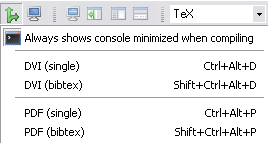
\includegraphics[scale=0.50]{./res/1_19_2_3.png}
  \end{quotation}
\end{footnotesize}


\subsection{1.19.2.2 (Feb/22/2007)}

\begin{itemize}
  \item Parts of the source code were optimized.
\end{itemize}


\subsection{1.19.2.1 (Feb/19/2007)}

\begin{itemize}
  \item Parts of the source code were optimized.
  \item The first approach to a easy \RR{} package manager was implemented:

\end{itemize}

\begin{footnotesize}
  \begin{quotation}
    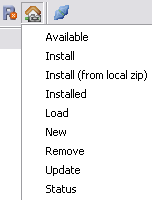
\includegraphics[scale=0.50]{./res/1_19_2_1.png}
  \end{quotation}
\end{footnotesize}

\begin{itemize}
  \item To avoid \RR{} flicker, if TCP/IP connection is active and
    the \textit{R output} is visible, the \textit{Clear console (F9)}
    and \textit{Clear all (F12)} will not work on the \RR{} console.
    We will be searching for the best solution.
\end{itemize}


\subsection{1.19.2.0 (Feb/16/2007)}

\begin{itemize}
  \item Bug(s) fixed:
    \begin{itemize}
      \item A bug related to the prior version and \textit{R toolbar} was fixed.
    \end{itemize}
\end{itemize}


\subsection{1.19.1.13 (Feb/13/2007)}

\begin{itemize}
  \item Bug(s) fixed:
    \begin{itemize}
      \item A bug that occurred when organizing the \textit{main toolbar},
        in the first use, was fixed.
    \end{itemize}
  \item Parts of the source code were optimized.
  \item An experimental graphical interface for tags was added to the
    program. It was made by adding a new tab named \textit{Tags} on
    the panel \textit{Tools} and it will aid the user to write Txt2tags,
    TeX, HTML and others from Tinn-R in graphical mode. In the current
    version only Txt2tags interface was implemented.
  \item The structure of the \textit{Tinn.ini} file was a bit reworked.
    So, the old backups will not be compatible anymore with this and
    future versions. This version will recognize the basic old system
    configurations, but not all preferences. Sorry for the inconvenience.
  \item The main menu \textit{View/Tools} was a bit reworked and has new
    resources.
  \item The \textit{Tools} window has now a new pop-up. It enables you to choose
    the visible pages:
\end{itemize}

\begin{footnotesize}
  \begin{quotation}
    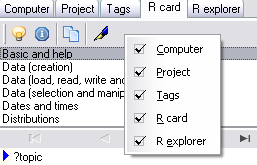
\includegraphics[scale=0.50]{./res/1_19_1_13.png}
  \end{quotation}
\end{footnotesize}


\subsection{1.19.1.12 (Feb/11/2007)}

\begin{itemize}
  \item \textit{Search} and \textit{Replace} interface was a bit reworked.
\end{itemize}


\subsection{1.19.1.11 (Feb/07/2007)}

\begin{itemize}
  \item Bug(s) fixed:
    \begin{itemize}
      \item A bug related to the prior version and \textit{R toolbar} (flicker) was fixed.
    \end{itemize}
\end{itemize}


\subsection{1.19.1.10 (Feb/04/2007)}

\begin{itemize}
  \item Parts of the source code were optimized.
  \item The \texttt{Tinn-R card} was updated.
  \item The \textit{Application options} interface was a bit reworked
    and the \textit{R resource visibles} was enhanced. Now if this option
    is not marked, all \RR{} resources will not be visible.
  \item A new option was added to the main menu \textit{View:
      \RR{} resources visible}.
\end{itemize}


\subsection{1.19.1.9 (Jan/25/2007)}

\begin{itemize}
  \item Bug(s) fixed:
    \begin{itemize}
      \item A bug related to \textit{R toolbar} was fixed.
    \end{itemize}
  \item Parts of the source code were optimized.
\end{itemize}


\subsection{1.19.1.8 (Jan/24/2007)}

\begin{itemize}
  \item Parts of the source code were optimized.
\end{itemize}


\subsection{1.19.1.7 (Jan/23/2007)}

\begin{itemize}
  \item Bug(s) fixed:
    \begin{itemize}
      \item Bugs related to selection in 'smLine' mode, were fixed.
        Many thanks to \texttt{SynEdit team}.
    \end{itemize}
  \item Parts of the source code were optimized.
  \item The main component \textit{SynEdit} was updated to the latest version.
\end{itemize}


\subsection{1.19.1.6 (Jan/21/2007)}

\begin{itemize}
  \item Bug(s) fixed:
    \begin{itemize}
      \item A bug related to the project interface was fixed.
      \item Small bugs, related to the editor in split mode
        (vertical or horizontal), were fixed.
    \end{itemize}
  \item Parts of the source code were optimized.
\end{itemize}


\subsection{1.19.1.5 (Jan/09/2007)}

\begin{itemize}
  \item Parts of the source code were optimized.
  \item Small adjustments were made to the program interface.
\end{itemize}


\subsection{1.19.1.4 (Jan/05/2007)}

\begin{itemize}
  \item Parts of the source code were optimized.
  \item The use of clipboard between \RR{} and Tinn-R was enhanced.
    For example, instructions such as the ones below are now possible:


    \begin{Scode}
      a <- round(rnorm(1000), 2)
      b <- round(rnorm(1000), 2)
      c <- round(rnorm(1000), 2)
      d <- data.frame(a, b, c)
      write.table(d, file="clipboard")
    \end{Scode}

    Tinn-R is frozen until \RR{} releases the clipboard. Thanks to
    \texttt{Igor Kojanov} for pointing out the problem and the soluction's direction.
  \item In the first use of the program, default options were changed.
  \item The \textit{R/Database} interface was reworked:
    \begin{itemize}
      \item A new option enabling the user to restore the original database
        was added.
      \item After changes it is necessary to type \textit{Save}. Otherwise, a
        ll changes will be lost when closing the interface.
      \item The button \textit{Save and close} was removed.
    \end{itemize}
\end{itemize}


\subsection{1.19.1.3 (Jan/04/2007)}

\begin{itemize}
  \item Parts of the source code were optimized.
  \item Menu \textit{R} was a bit reworked.
  \item Icons were changed.
  \item In the first use of the program, default options were changed.
  \item The \textit{R/Database} interface was a bit reworked. It now
    has a new option enabling the user to restore the original database.
\end{itemize}


\subsection{1.19.1.2 (Jan/01/2007)}

\begin{itemize}
  \item The menu \textit{R} was a bit reworked and now has a new option:
    \textit{Customize}. It enables the user to customize the files
    \texttt{Rcompletion.r} and \texttt{Rconfigure.r}. Before that,
    administrator privileges were necessary to personalize these
    very useful files.
  \item The folder where Tinn-R stores its internal files has now a
    new sub-folder named \textit{custom} that stores the files
    \texttt{Rcompletion.r} and \texttt{Rconfigure.r}. It will be
    also included in backups of the system configuration.
\end{itemize}
